\documentclass[11pt]{article}
\pagestyle{empty}
%\usepackage[latin1]{inputenc}
\usepackage[utf8]{inputenc}
\usepackage{a4wide}
\usepackage{amsmath}
\usepackage{amssymb}
\usepackage{amsthm}
\usepackage{german}
\usepackage{multirow,array}
\usepackage{hyperref}
 \usepackage{graphicx}
%\usepackage{ipe}
%\input{thmstyle-ger}

\parindent0mm
\sloppy

% Basic data
\newcommand{\VORLESUNG}{Induktive Statistik für Soziologinnen und Soziologen}
\newcommand{\STAFF}{Mariana Nold}
\newcommand{\ASSIGNMENT}{1}
\newcommand{\HANDOUT}{Montag, den 23.Oktober   2017}
\newcommand{\DELIVER}{keine Abgabe, wird in der Übung besprochen}
\newcommand{\PRACTICAL}[1]{\marginpar{\tiny {\bf Aufgabe \\ abgeben!} #1}}
\newcommand{\FAUFTRAG}[1]{\marginpar{\tiny {\bf selbst entdeckendes Verstehen} #1}}
\newcommand{\titel}{Zufallsvorgang, Inferenzschluss und Wahrscheinlichkeitsverteilungen}
\newcommand{\startwert}{0}

% Arbitrary packages and settings

\newcommand{\N}{\mathbb{N}}
\newcommand{\floor}[1]{\lfloor{#1}\rfloor}
\newcommand{\ceil}[1]{\lceil{#1}\rceil}
\newcommand{\half}[1]{\frac{#1}{2}}
\newcommand{\punkte}[1]{{\small{ }(#1 Punkte)}}
\newcommand{\punkt}[1]{{\small{ }(#1 Punkt)}}

\newcommand{\aufgabe}[1]{\item{\bf #1}}
\newcommand{\hinweis}{{\em Hinweis}}

\begin{document}
% Document title

\begin{center}
\ASSIGNMENT{}. Übungsblatt vom \HANDOUT{} zur Vorlesung 
\vspace*{0.5cm}

{\Large \VORLESUNG{}}
%\PRACTICAL{}
(\STAFF{}) 


\vspace*{0.5cm}
{\textbf{Thema:} \titel{}\\}
\vspace*{0.2cm}

{\small Abgabe: \DELIVER{}}
\vspace*{1cm}
\end{center}

Wichtige Definitionen:
\begin{enumerate}
\item{Zufallsvorgang}
\item{Zufallsvariable}
\item{Einfache Zufallsstichprobe}
\item{Wahrscheinlichkeitsverteilung}
\item{Binäre Variable und  Bernoulliverteilung}
\item{Binomialverteilung}
\end{enumerate}
\vspace{2cm}
\begin{enumerate}\addtocounter{enumi}{\startwert}






\aufgabe{Relative Häufigkeit beim Münzwurf}

In der Vorlesung hatten wir die Wahrscheinlichkeitsfunktion der Binomialverteilung für den
$10$-fachen Münzwurf kennen gelernt. Die entsprechend Grafik ist gegeben durch
Abbildung \ref{abb1}. Die Tabelle \ref{tab1} enthält die entsprechenden Werte in Zahlen.

 \begin{figure}[ht]
 	\centering
 	      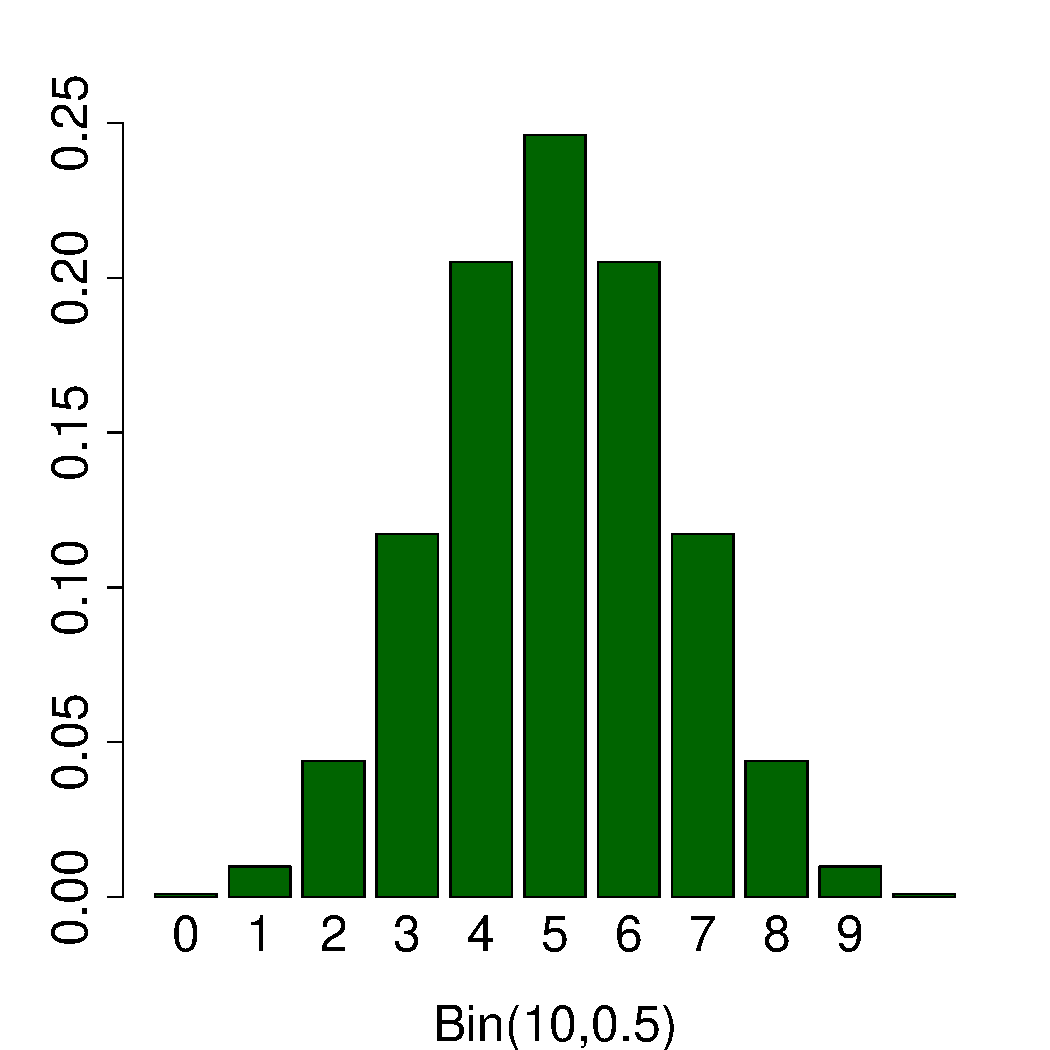
\includegraphics[width=0.55\textwidth]{muenze.pdf}
 	      \caption{Wahrscheinlichkeitsfunktion der Binomialverteilung $p=0.5$ und $n=10$
 	       \label{abb1}}
 	\end{figure}
 	
 	Diese Wahrscheinlichkeitsfunktion  lässt sich auch in Form einer Tabelle angeben
 	% 0.001 0.010 0.044 0.117 0.205 0.246 0.205 0.117 0.044 0.010 0.001
 	 \begin{table}[h]
 \centering 
 \small
\begin{tabular}{|r|r|r|r|r|r|r|r|r|r|r|r|}
  \hline
   Anzahl Treffer  $y$                               & $0$    &   $1$    & $2$   & $3$   & $4$   & $5$ &   $6$    & $7$   & $8$   & $9$   & $10$\\ \hline
   W'keit $\mathbb{P}(Y=y)$ & $0.001$ & $0.010$ & $0.044$ & $0.117$ & $0.205$ & $0.246$ & $0.205$ & $0.117$ & $0.044$ & $0.010$ & $0.001$  \\ \hline
\end{tabular}
 \caption{Wahrscheinlichkeitsfunktion der $Bin(n=10,p=0.5)$-Verteilung \label{tab1}}
 \end{table}  


\begin{enumerate}
\item{Nehmen Sie an, dass $200$ Studierende an dem Experiment $10$-facher Münzwurf teilgenommen haben.  Jede Person hat $10$ Mal eine Münze
geworfen und die Anzahl der Treffer (Münze zeigt Zahl) auf einem Zettel notiert. Warum handelt es sich um einen Zufallsvorgang?}
\item{Nutzen Sie die Zufallsvariable $Y,$ um den Zufallsvorgang formal zu beschreiben.}
\item{Sie wählen zufällig eine Person von diesen $200$ Studierenden aus und fragen sie, ob sie auf ihrem Zettel die Zahl $4$ notiert hat. Wie hoch ist die Wahrscheinlichkeit,
dass die Person mit ``ja'' antwortet?}
\item{Nach welcher Zahl $y$ müssen Sie fragen, damit ihre Wahrscheinlichkeit eine Ja-Antwort zu bekommen maximal ist?}
\item{Beruhend auf den Überlegungen in Teilaufgabe d): Wo liegt der Modus der Wahrscheinlichkeitsfunktion der $Bin(n=10,p=0.5)$-Verteilung?}
\item{Wie hoch ist die Wahrscheinlichkeit, dass eine zufällig ausgewählte Person tatsächlich $10$ Mal in Folge einen Treffer erzielt hat?}
\item{Sie bitten alle Studierenden, die genau einen Treffer erzielt haben, sich zu melden. Wie viele Meldungen erwarten Sie beruhend auf
den Angaben in Tabelle \ref{tab1}. }
\item{Wie viele Meldungen erwarten Sie beruhend auf
den Angaben in Tabelle \ref{tab1}, wenn Sie alle Studierenden bitten, sich zu melden, die genau sechs Treffer erzielt haben?}
\end{enumerate}

\aufgabe{Erwartungswert und Mittelwert  beim Münzwurf}
In dieser Aufgabe betrachten wir nochmal den Zufallsvorgang aus Aufgabe 1. $200$ Studierende werfen je $10$ Mal eine Münze.
Es sei 
\begin{equation*}
Y_{i} := \text{Anzahl der Treffer bei $10$ Münzwürfen der Person $i$} i \in \{0,\dots 200\}
\end{equation*}
Endsprechen bezeichnet $y_{i}$ die Anzahl der Treffer die Person $i$ erzielt hat. So beinhaltet z. B. $y_{3}=8$
die Information, dass die dritte Person genau acht Treffer erzielt hat.

Sie kennen aus dem letzten Semester das arithmetische Mittel $\bar{y}.$ Es wird berechnet als
\begin{equation*}
\bar{y} = \sum_{i=1}^{n=200} y_{i}.
\end{equation*}
Die Abbildung \ref{abb2} zeigt die relative Häufigkeitsverteilung die bei der Durchführung des Zufallsvorgangs beobachtet wurde.
% 0  0  4 18 43 56 47 26  3  3  0
 \begin{figure}[ht]
 	\centering
 	      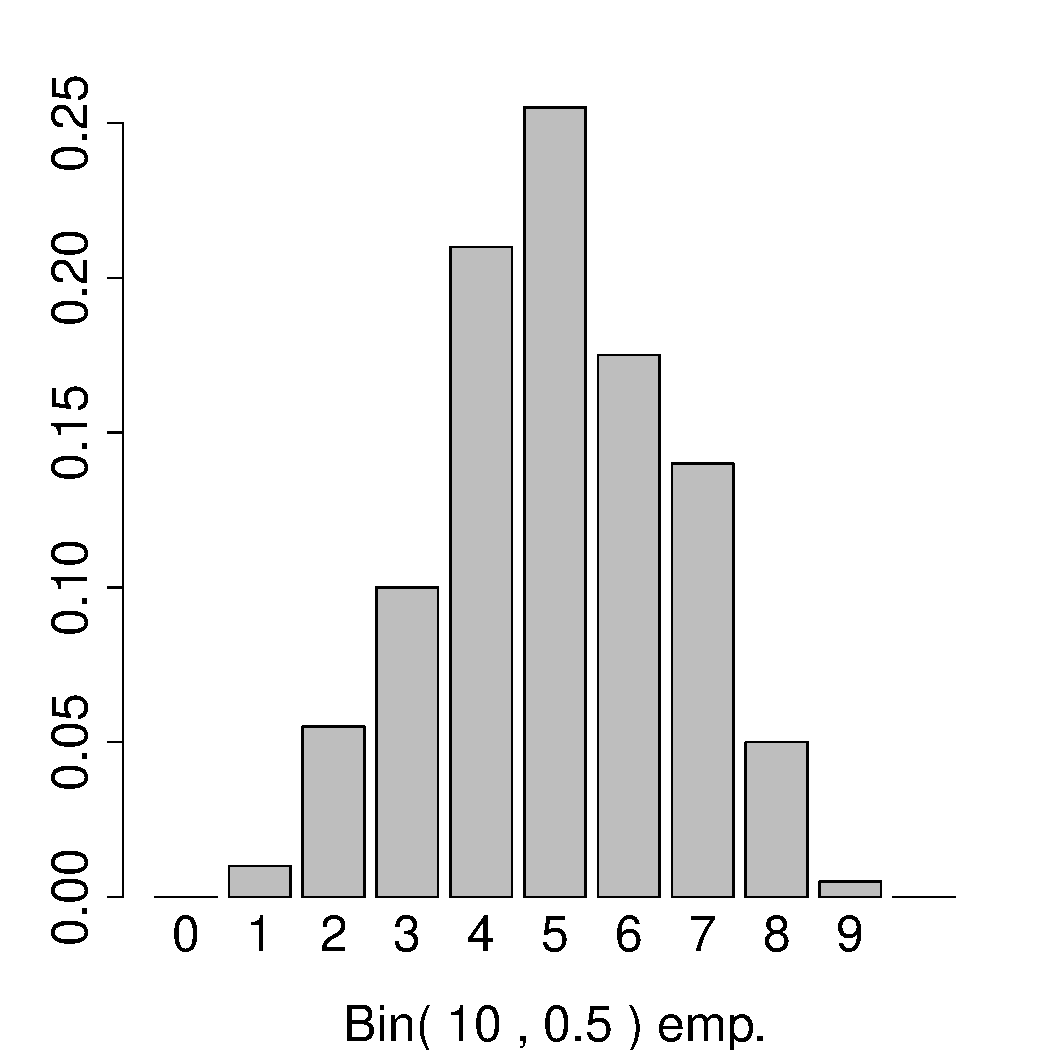
\includegraphics[width=0.55\textwidth]{muenzeEmp.pdf}
 	      \caption{Wahrscheinlichkeitsfunktion der Binomialverteilung $p=0.5$ und $n=10$
 	       \label{abb2}}
 	\end{figure}
 	
 	\begin{table}[h]
 	 \centering 
 \small %0.000 0.000 0.020 0.090 0.215 0.280 0.235 0.130 0.015 0.015 0.000
\begin{tabular}{|r|r|r|r|r|r|r|r|r|r|r|r|}
  \hline
   Anzahl Treffer  $y$                               & $0$    &   $1$    & $2$   & $3$   & $4$   & $5$ &   $6$    & $7$   & $8$   & $9$   & $10$\\ \hline
   rel. H'keit & $0.000$ & $0.000$ & $0.020$ & $0.090$ & $0.215$ & $0.280$ & $0.235$ & $0.130$ & $0.015$ & $0.015$ & $0.000$  \\ \hline
    abs. H'keit & $0$ & $0$ & $4$ & $18$ & $43$ & $56$ & $47$ & $26$ & $3$ & $3$ & $0$  \\ \hline
\end{tabular}
 \caption{rel. Häufigkeit die beim Zufallsvorgang $10$-facher Münzwurf von $200$ Personen beobachtet wurde. \label{tab2}}
 \end{table}  


\begin{enumerate}
\item{Warum sind Abbildung \ref{abb1} und Abbildung \ref{abb2} ähnlich aber nicht gleich? Worin ähneln die beiden Abbildungen sich
und wo sehen Sie Unterschiede? Zur besseren Vergleichbarkeit enthält Tabelle \ref{tab2} die relativen Häufigkeiten, die in Abbildung
\ref{abb2} dargestellt sind.}
\item{Vergleichen Sie die erwartete Anzahl der Meldungen aus  Aufgabe 1 g) und 1 h) mit den tatsächlich beobachteten Häufigkeiten.}
\item{Welcher Zusammenhang besteht zwischen der absoluten und der relativen Häufigkeit?}
\item{Nutzen Sie die absolute Häufigkeit aus Tabelle \ref{tab2} um den Mittelwert $\bar{y}$ zu berechnen und interpretieren Sie diesen Wert.}
\item{Wie kann das arithmetische Mittel $\bar{y}$ beruhend auf den relativen Häufigkeiten berechnet werden?}
\item{Nutzen Sie den gleichen Rechenansatz wie in Teilaufgabe e) um den Erwartungswert der $Bin(n=10,p=0.5)$-Verteilung zu berechnen.
empfohlene Literatur: W. Ludwig-Mayerhofer, Statistik S. 104-106}
\end{enumerate}
% https://www.beratung-statistik.de/statistik-beratung-infos/stata-tutorial/regression-stata-interpretation/
%https://www.stata.com/statalist/archive/2008-06/msg00018.html
%https://www.beratung-statistik.de/statistik-beratung-infos/stata-tutorial/stata-nachhilfe-zufallszahlen/
\newpage
\aufgabe{Analyse der Daten mit \texttt{STATA}} % Müssen Sie selber machen
Lesen Sie den Datensatz \texttt{munze.dta} ein.
\begin{enumerate}
\item{Nutzen Sie den Befehlt \texttt{. summarize} um eine Zusammenfassung der Daten zu erhalten.}
\item{Nutzen Sie den Befehlt \texttt{. tab AnzTreffer} um eine Tabelle der Daten zu erhalten.}
\item{Lesen Sie aus der in Teilaufgabe e) erzeugten Tabelle ab, wie hoch der Anteil der Studierenden ist,
der höchstens sechs Treffer erzielt hat.}
\item{Nutzen Sie den Befehl  \texttt{. graph box AnzTreffer} um einen Boxplot zu erstellen und beschreiben Sie diesen Boxplot in Worten.}
\end{enumerate}

\end{enumerate}
\end{document}
